\documentclass[conference]{IEEEtran}
\IEEEoverridecommandlockouts
\usepackage[utf8]{inputenc}
\usepackage[T1]{fontenc}
\usepackage[brazilian]{babel}
\usepackage{cite}
\usepackage{amsmath,amssymb,amsfonts}
\usepackage{graphicx}
\usepackage{textcomp}
\usepackage{xcolor}
\usepackage{booktabs}
\usepackage{placeins}
\usepackage{float}
\newcommand{\pl}{\ensuremath{+}}
\newcommand{\mn}{\ensuremath{-}}
\def\BibTeX{{\rm B\kern-.05em{\sc i\kern-.025em b}\kern-.08em
    T\kern-.1667em\lower.7ex\hbox{E}\kern-.125emX}}
\begin{document}

\title{Imagens Sintéticas de uma DCGAN Ajudam a Detectar Dermatofibroma? Uma Avaliação Controlada no ISIC 2019}

\author{\IEEEauthorblockN{1\textsuperscript{st} José Joaquim da Silva Neto}
\IEEEauthorblockA{\textit{Faculdade de Ciências e Tecnologias em Engenharia} \\
\textit{Universidade de Brasília (UnB)}\\
Brasília, Brasil \\
netojoaquimjj@gmail.com \\
Matrícula: 232027510}
\and
\IEEEauthorblockN{2\textsuperscript{nd} Pedro Henrique Gomes}
\IEEEauthorblockA{\textit{Faculdade de Ciências e Tecnologias em Engenharia} \\
\textit{Universidade de Brasília (UnB)}\\
Brasília, Brasil \\
pedrohg2609@gmail.com \\
Matrícula: 232030041}
}

\maketitle

\begin{abstract}
O diagnóstico dermatológico assistido por inteligência artificial depende de dados raramente balanceados, e lesões raras aparecem em poucos exemplos. Este trabalho avalia se imagens sintéticas geradas por uma Deep Convolutional GAN (DCGAN) ajudam um classificador ResNet18 a detectar o dermatofibroma (DF), a classe mais rara do ISIC~2019, com 239 de 25\,331 imagens. O protocolo evita vazamento de informação: em cada um dos 5 \textit{folds} de validação cruzada, a GAN é treinada do zero apenas com as DF do conjunto de treino, e a época e o limiar do classificador são escolhidos na validação. O desempenho é medido sobre todas as 239 DF, com 3 sementes por \textit{fold} e intervalos de confiança \textit{bootstrap} pareados. Sete condições são comparadas, incluindo réplicas de imagens reais, peso na perda e amostragem balanceada como controles. As imagens sintéticas isoladas não melhoraram a detecção, com variação de recall de \pl0,008 (intervalo de \mn0,026 a \pl0,040), e combinadas a outras estratégias também não trouxeram ganho mensurável. Já repetir imagens reais de DF e ponderar a perda elevaram o recall em 0,071 e 0,061. Por subgrupo, o recall é menor nos homens (0,47 contra 0,62 no \textit{baseline}) e nenhuma condição corrigiu a diferença. A GAN obteve FID entre 191 e 225 e baixa diversidade, de modo que o resultado vale para este gerador e não descarta ganhos com geradores melhores.
\end{abstract}

\begin{IEEEkeywords}
GAN, DCGAN, dermatofibroma, ISIC 2019, desbalanceamento de classes, equidade, aumento de dados.
\end{IEEEkeywords}

\section{Introdução}
O aprendizado profundo alcançou desempenho competitivo na análise de imagens dermatoscópicas, em grande parte graças a coleções públicas como HAM10000 e ISIC \cite{tschandl2018ham10000,codella2018skin,combalia2019bcn20000}. Essas coleções, porém, refletem a prevalência clínica das lesões. Os nevos melanocíticos dominam, enquanto condições raras, como o dermatofibroma, aparecem em poucas centenas de exemplos diante de cerca de 25 mil imagens.

Esse desequilíbrio tem consequências para a equidade (\textit{fairness}). Um modelo que raramente vê uma condição durante o treino tende a não detectá-la, e o custo recai sobre os pacientes que a apresentam. Disparidades de desempenho em IA dermatológica já foram documentadas \cite{daneshjou2022disparities}, e métricas agregadas como a acurácia escondem essa falha, pois a classe rara pesa pouco no total.

Uma resposta comum é aumentar os dados. Rotações e espelhamentos, no entanto, apenas reorganizam a informação já disponível, ao passo que as Redes Adversárias Generativas (GANs) \cite{goodfellow2014generative} aprendem a distribuição das imagens e, em princípio, podem produzir exemplos novos, com resultados positivos já relatados em imagens médicas \cite{frid2018gan}. Este trabalho testa essa hipótese para o DF de forma controlada. Três cuidados orientam o desenho. A GAN vê apenas imagens do conjunto de treino de cada \textit{fold}. As imagens sintéticas são comparadas a controles que adicionam o mesmo número de amostras sem informação nova e a técnicas padrão de rebalanceamento \cite{buda2018systematic}. E cada diferença é acompanhada de um intervalo de confiança.

\section{Metodologia}

\subsection{Base de Dados e Partições}
Utilizou-se o ISIC~2019 na versão do Kaggle, com 25\,331 imagens dermatoscópicas de treino e oito classes diagnósticas. A Tabela~\ref{tab:dados} contrasta a classe majoritária, nevo melanocítico (NV), com a minoritária, DF. A contagem de DF (239) foi obtida dos metadados, e as demais seguem a distribuição oficial do desafio \cite{combalia2019bcn20000}. Todas as imagens foram reduzidas a 64$\times$64 por interpolação bilinear.

\begin{table}[ht]
\centering
\caption{Amostras por classe no ISIC 2019 (treino)}
\label{tab:dados}
\small
\begin{tabular}{lrr}
\toprule
\textbf{Classe} & \textbf{Imagens} & \textbf{Proporção} \\
\midrule
NV (majoritária) & 12\,875 & 50,8\% \\
MEL & 4\,522 & 17,9\% \\
BCC, BKL, AK, SCC, VASC & 7\,695 & 30,4\% \\
DF (minoritária) & 239 & 0,9\% \\
\midrule
Total & 25\,331 & 100\% \\
\bottomrule
\end{tabular}
\end{table}

A avaliação usa validação cruzada estratificada em 5 \textit{folds}, com o rótulo DF contra o resto. Em cada \textit{fold}, o conjunto de treino é dividido de novo para separar um sexto como validação. Isso resulta em cerca de 16\,900 imagens de treino (de 154 a 163 DF), 3\,400 de validação e 5\,070 de teste. Cada imagem aparece no teste exatamente uma vez, de modo que as métricas finais cobrem as 25\,331 imagens e as 239 DF. O arquivo de treino do Kaggle não traz identificador de lesão (o metadado oficial traz, mas ele não foi usado na divisão), de modo que esta é feita por imagem. A consequência é discutida na Seção~\ref{sec:disc}.

\subsection{Arquitetura da DCGAN}
A arquitetura segue a DCGAN de Radford~\textit{et~al.}~\cite{radford2016unsupervised}. O \textbf{gerador} recebe um vetor latente $z\in\mathbb{R}^{100}$ e o amplia por cinco camadas \texttt{ConvTranspose2d} de núcleo 4$\times$4 (512, 256, 128, 64 e 3 canais). As camadas intermediárias usam \textit{BatchNorm} e ReLU, e a saída usa Tanh, resultando em imagens de 64$\times$64$\times$3 em $[-1,1]$. O \textbf{discriminador} espelha esse desenho com cinco camadas \texttt{Conv2d} de \textit{stride}~2 (64, 128, 256 e 512 filtros e, por fim, um canal de saída), sem \textit{max pooling}, com \textit{BatchNorm} e LeakyReLU de inclinação 0,2. Os pesos convolucionais seguem uma normal de desvio-padrão 0,02, e a sigmoide está embutida na função de custo (\texttt{BCEWithLogitsLoss}), de modo que o discriminador emite um \textit{logit}.

\subsection{Treinamento da GAN}
Uma GAN independente é treinada do zero em cada \textit{fold}, usando somente as DF do conjunto de treino (de 154 a 163 imagens). A função de custo é a entropia cruzada binária do treinamento adversário \cite{goodfellow2014generative}, otimizada com Adam \cite{kingma2015adam}, taxa de aprendizado $2\times10^{-4}$ e $\beta_1=0{,}5$ nas duas redes, por 4000 iterações com lotes de 64. Como o conjunto é muito pequeno, três recursos ajudam a estabilizar a disputa entre gerador e discriminador: (i) suavização dos rótulos reais para 0,9 \cite{salimans2016improved}, (ii) aumento diferenciável de dados (DiffAugment \cite{zhao2020differentiable}, com cor, translação e \textit{cutout}, além de espelhamentos) aplicado às imagens reais e falsas antes do discriminador e (iii) média móvel exponencial dos pesos do gerador, com fator 0,999 \cite{yazici2019unusual}. A cada 250 iterações mede-se o FID entre 1000 amostras e as DF de treino, e o ponto de menor FID é mantido. As DF de validação e de teste não participam da GAN nem dessa escolha.

\subsection{Avaliação da GAN}
A fidelidade é medida pelo FID \cite{heusel2017gans}, calculado sobre as \textit{features} da Inception com os pesos do \texttt{pytorch-fid} \cite{seitzer2020pytorchfid}. Reporta-se o FID de 1000 amostras contra as DF de treino e, apenas como informação, contra as DF fora do treino. Para checar memorização, mede-se para 300 amostras a distância ao vizinho mais próximo entre as DF de treino, nas \textit{features} de uma ResNet18 pré-treinada, e compara-se sua mediana com a de DF não vistas até as DF de treino.

\subsection{Classificador e Condições}
O classificador é uma ResNet18 \cite{he2016deep} pré-treinada na ImageNet, para a tarefa binária DF contra o resto. Todas as imagens, reais e sintéticas, entram em 64$\times$64 e são ampliadas a 112$\times$112, para que as sintéticas não se distingam apenas por borramento. O treino usa espelhamentos, Adam com taxa de $10^{-4}$ e decaimento cosseno, 8 épocas e lotes de 128. A época é escolhida pela PR-AUC na validação e o limiar de decisão pelo F1 na validação, e o teste só é usado depois dessas escolhas. Sete condições são comparadas, cada uma com 3 sementes por \textit{fold}:
\textit{Baseline} (dados originais), \textit{Controle} (mais 1000 réplicas de DF reais), \textit{+GAN} (mais 1000 sintéticas), \textit{Controle+GAN} (ambas), \textit{Peso} (peso positivo $\sqrt{n_\text{neg}/n_\text{pos}}$ na perda), \textit{Amostragem} (amostragem balanceada por classe) e \textit{Amostragem+GAN} (amostragem balanceada com 1000 sintéticas).

As predições de teste dos 5 \textit{folds} são agrupadas e avaliadas por recall, precisão e F1 no limiar da validação, e por AUC e PR-AUC. Os intervalos de confiança de 95\% vêm de \textit{bootstrap} estratificado por imagem (1000 reamostragens) e são pareados.

\section{Resultados}

\subsection{Qualidade da GAN}
\begin{figure}[!t]
\centering
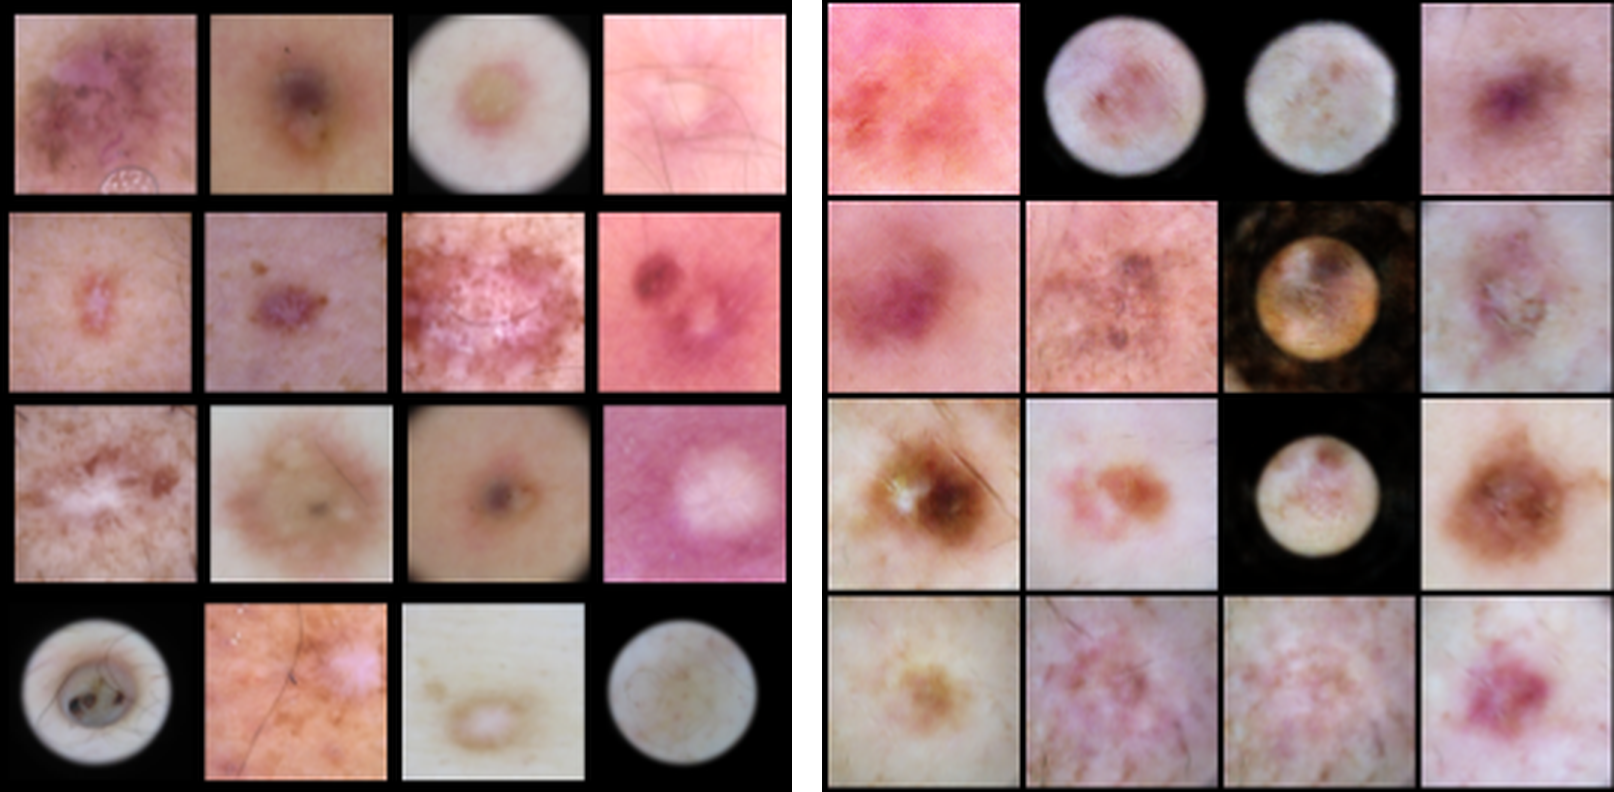
\includegraphics[width=\linewidth]{fig_grids.png}
\caption{Esquerda: DF reais do treino (64$\times$64). Direita: DF sintéticas do \textit{fold}~0.}
\label{fig:grids}
\end{figure}

\begin{figure}[!t]
\centering
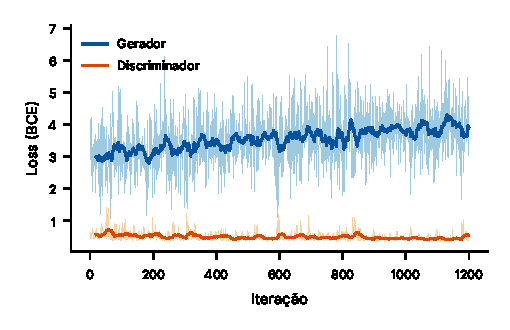
\includegraphics[width=\linewidth]{fig_loss.pdf}
\caption{Perdas por iteração no \textit{fold}~0 (traços claros) e média móvel de 20 iterações (traços escuros).}
\label{fig:loss}
\end{figure}

A Fig.~\ref{fig:grids} compara DF reais do treino com sintéticas no \textit{fold}~0. A GAN reproduz a cor da pele, a mancha central e o campo circular escuro de alguns dermatoscópios, mas as imagens são borradas e exibem uma textura periódica artificial, sem pelos nem bordas nítidas. A Fig.~\ref{fig:loss} mostra as perdas desse \textit{fold}. Depois de um transiente inicial, ficam estáveis em torno de 1,3 para o discriminador e 1,1 para o gerador, sem divergência, e a perda do discriminador permanece perto de $2\ln 2\approx1{,}39$, valor de quem não distingue reais de falsas.

O FID dos pontos escolhidos ficou entre 191 e 225 (média 207,6) contra as DF de treino e entre 207 e 249 (média 225,3) contra as DF fora do treino, valores altos que confirmam a qualidade limitada. Em 3 dos 5 \textit{folds} a melhor iteração foi a última (4000), de modo que o FID ainda caía ao fim do treino. Quanto à memorização, a mediana da distância das sintéticas às DF de treino foi 8,38 em média, acima da mediana das DF não vistas (7,36), e a razão ficou acima de 1 em 4 dos 5 \textit{folds} (média 1,14) e em 0,95 no restante. Não há, portanto, indício consistente de cópia. A Fig.~\ref{fig:nn}, porém, revela baixa diversidade: no \textit{fold}~0, 7 das 8 sintéticas têm como vizinha uma entre apenas duas imagens reais.

\subsection{Impacto no classificador}
A Tabela~\ref{tab:clf} resume as sete condições. O \textit{baseline} já detecta cerca de metade das DF, com recall de 0,544, precisão de 0,674 e PR-AUC de 0,621. Repetir imagens reais (\textit{Controle}) elevou o recall a 0,615, um ganho de 0,071 com intervalo de 0,036 a 0,109 (Tabela~\ref{tab:diff}), e a PR-AUC em 0,032, ao custo de uma queda de 0,024 na AUC. O peso na perda teve efeito semelhante sobre o recall (\pl0,061) e deu a maior AUC (0,959). A amostragem balanceada não trouxe ganho claro (\pl0,021, intervalo de \mn0,013 a \pl0,056).

As imagens sintéticas, por sua vez, não mudaram o desempenho de forma mensurável. Adicionadas ao \textit{baseline}, deixaram o recall praticamente igual (\pl0,008, intervalo de \mn0,026 a \pl0,040) e reduziram a precisão em 0,049 (intervalo de \mn0,090 a \mn0,009). Combinadas às réplicas, o recall caiu 0,027 (intervalo de \mn0,056 a \pl0,001) e a precisão subiu 0,045 (intervalo de 0,006 a 0,082), sem alterar o F1 (\pl0,005, intervalo de \mn0,021 a \pl0,032). Com a amostragem balanceada, a adição de imagens sintéticas também não alterou o recall (\mn0,013, intervalo de \mn0,039 a \pl0,013).

\begin{table}[ht]
\centering
\caption{Desempenho no teste (25\,331 imagens, 239 DF), média de 3 sementes. O desvio-padrão entre sementes é de no máximo 0,05.}
\label{tab:clf}
\scriptsize
\setlength{\tabcolsep}{3pt}
\begin{tabular}{lccccc}
\toprule
\textbf{Condição} & \textbf{Recall} & \textbf{Prec.} & \textbf{F1} & \textbf{AUC} & \textbf{PR-AUC} \\
\midrule
Baseline & 0,544 & 0,674 & 0,602 & 0,949 & 0,621 \\
Controle & \textbf{0,615} & 0,641 & 0,627 & 0,925 & \textbf{0,653} \\
+ GAN & 0,552 & 0,627 & 0,587 & 0,948 & 0,611 \\
Controle + GAN & 0,589 & \textbf{0,686} & \textbf{0,632} & 0,913 & 0,636 \\
Peso na perda & 0,605 & 0,622 & 0,612 & \textbf{0,959} & 0,618 \\
Amostragem & 0,565 & 0,620 & 0,591 & 0,917 & 0,605 \\
Amostragem + GAN & 0,552 & 0,658 & 0,599 & 0,927 & 0,605 \\
\bottomrule
\end{tabular}
\end{table}

\begin{table}[ht]
\centering
\caption{Diferenças pareadas (A $-$ B) com IC 95\% bootstrap. Em negrito, intervalos que não contêm zero.}
\label{tab:diff}
\scriptsize
\setlength{\tabcolsep}{2pt}
\begin{tabular}{lcc}
\toprule
\textbf{A $-$ B} & \textbf{Recall} & \textbf{PR-AUC} \\
\midrule
+GAN $-$ Baseline & \pl0,008 (\mn0,026 a \pl0,040) & \mn0,009 (\mn0,036 a \pl0,017) \\
Controle+GAN $-$ Controle & \mn0,027 (\mn0,056 a \pl0,001) & \mn0,016 (\mn0,039 a \pl0,005) \\
Controle $-$ Baseline & \textbf{\pl0,071 (\pl0,036 a \pl0,109)} & \textbf{\pl0,032 (\pl0,005 a \pl0,058)} \\
Peso $-$ Baseline & \textbf{\pl0,061 (\pl0,031 a \pl0,091)} & \mn0,003 (\mn0,024 a \pl0,017) \\
\bottomrule
\end{tabular}
\end{table}

\subsection{Análise por subgrupo}
Com o metadado oficial (sexo, idade aproximada e região anatômica), calculou-se o recall por subgrupo a partir das mesmas predições, sem retreinar. A Tabela~\ref{tab:sub} mostra os grupos com ao menos 39 DF e quatro das sete condições. Não há DF entre as 4587 imagens de cabeça e pescoço. A DF concentra-se nos membros inferiores (138 de 239, prevalência de 2,8\%), contra 0,5\% no tronco.

\begin{table}[ht]
\centering
\caption{Recall por subgrupo (média de 3 sementes). Entre parênteses, o número de DF no teste.}
\label{tab:sub}
\scriptsize
\setlength{\tabcolsep}{2.2pt}
\begin{tabular}{lcccccccc}
\toprule
& \multicolumn{2}{c}{\textbf{Sexo}} & \multicolumn{3}{c}{\textbf{Idade (anos)}} & \multicolumn{3}{c}{\textbf{Região}} \\
\cmidrule(lr){2-3}\cmidrule(lr){4-6}\cmidrule(lr){7-9}
\textbf{Condição} & F & M & $<$40 & 40--59 & $\geq$60 & MI & MS & Tr. \\
& (117) & (122) & (39) & (121) & (79) & (138) & (52) & (45) \\
\midrule
Baseline & 0,62 & 0,47 & 0,65 & 0,47 & 0,61 & 0,57 & 0,49 & 0,57 \\
Controle & 0,69 & 0,54 & 0,68 & 0,56 & 0,66 & 0,63 & 0,60 & 0,60 \\
+ GAN & 0,63 & 0,48 & 0,67 & 0,49 & 0,59 & 0,59 & 0,49 & 0,53 \\
Peso na perda & 0,69 & 0,52 & 0,68 & 0,55 & 0,65 & 0,61 & 0,54 & 0,61 \\
\bottomrule
\end{tabular}
\end{table}

A disparidade mais clara é por sexo. No \textit{baseline}, o recall é 0,62 nas mulheres e 0,47 nos homens, uma diferença de 0,146 (IC 95\% de 0,036 a 0,249), e ela persiste em todas as condições, entre 0,146 e 0,191. Por idade, o grupo de 40 a 59 anos é o pior, com recall 0,18 abaixo dos menores de 40 (intervalo de 0,02 a 0,34) e 0,15 abaixo dos maiores de 60 (intervalo de 0,02 a 0,27) no \textit{baseline}, mas os intervalos passam a incluir zero em várias condições com rebalanceamento. Por região, os membros superiores ficam 0,08 abaixo dos inferiores, com intervalo de \mn0,06 a \pl0,22. As comparações são descritivas, pois os atributos são correlacionados e não houve correção para múltiplas comparações.

Quanto às imagens sintéticas, nenhum subgrupo mostrou ganho em relação ao \textit{baseline}, com variações entre \mn0,04 e \pl0,02 e todos os intervalos incluindo zero. As réplicas reais, ao contrário, elevaram o recall em ambos os sexos (\pl0,07 nos dois), nas idades de 40 a 59 (\pl0,10), nos membros inferiores (\pl0,06) e nos superiores (\pl0,11), todos com intervalo acima de zero. Nenhuma condição reduziu a diferença entre homens e mulheres.

\section{Discussão e Limitações}
\label{sec:disc}
O resultado central é negativo: nesta configuração, as imagens da DCGAN não melhoraram a detecção do DF. O intervalo da diferença de recall entre \textit{+GAN} e \textit{Baseline} (\mn0,026 a \pl0,040) exclui ganhos maiores que cerca de 4 pontos percentuais, mas não ganhos menores, e vale para o gerador usado, não para GANs em geral.

Três fatores provavelmente contribuem para isso. O primeiro é a qualidade, pois o FID entre 191 e 225 e as imagens borradas indicam que o gerador aprendeu cor e forma grosseiras, mas não a textura fina que caracteriza o DF. O segundo é a diversidade, já que a Fig.~\ref{fig:nn} sugere que as sintéticas se concentram em poucas regiões do espaço de \textit{features}, de modo que 1000 imagens trazem pouca informação além das cerca de 155 reais. O terceiro é a duração do treino, pois o FID ainda caía em 3 dos 5 \textit{folds} ao fim das 4000 iterações.

Treino mais longo ou em maior resolução pode alterar o resultado, o que não foi testado.

Os controles foram essenciais. Repetir imagens reais e ponderar a perda, técnicas que não trazem informação nova, aumentaram o recall em 0,07 e 0,06, ganhos que sem esses controles poderiam ter sido atribuídos às imagens sintéticas.

Há ainda limitações a considerar. A divisão por imagem permite que imagens da mesma lesão caiam em partições diferentes. Com o \texttt{lesion\_id} do metadado oficial, verificou-se que 60,3\% das imagens de teste (78,2\% das DF, 187 de 239) têm outra imagem da mesma lesão no treino ou na validação do seu \textit{fold}. Isso tende a inflar o desempenho absoluto de todas as condições, e a comparação entre condições é menos afetada, mas não está livre do problema. Repetir o experimento com divisão por lesão é o principal ajuste pendente. A resolução de 64$\times$64 descarta texturas usadas por dermatologistas. Cada \textit{fold} tem uma única GAN e 3 sementes por condição, e a escolha de época e de limiar usa poucas dezenas de DF de validação. Testou-se um único número de imagens extras (1000) e uma única configuração de GAN. Por fim, avaliou-se uma só classe rara e a análise por subgrupo cobre apenas sexo, idade e região, com poucas dezenas de DF por grupo e sem informação de tom de pele, indispensável para afirmações diretas sobre equidade.

\begin{figure}[H]
\centering
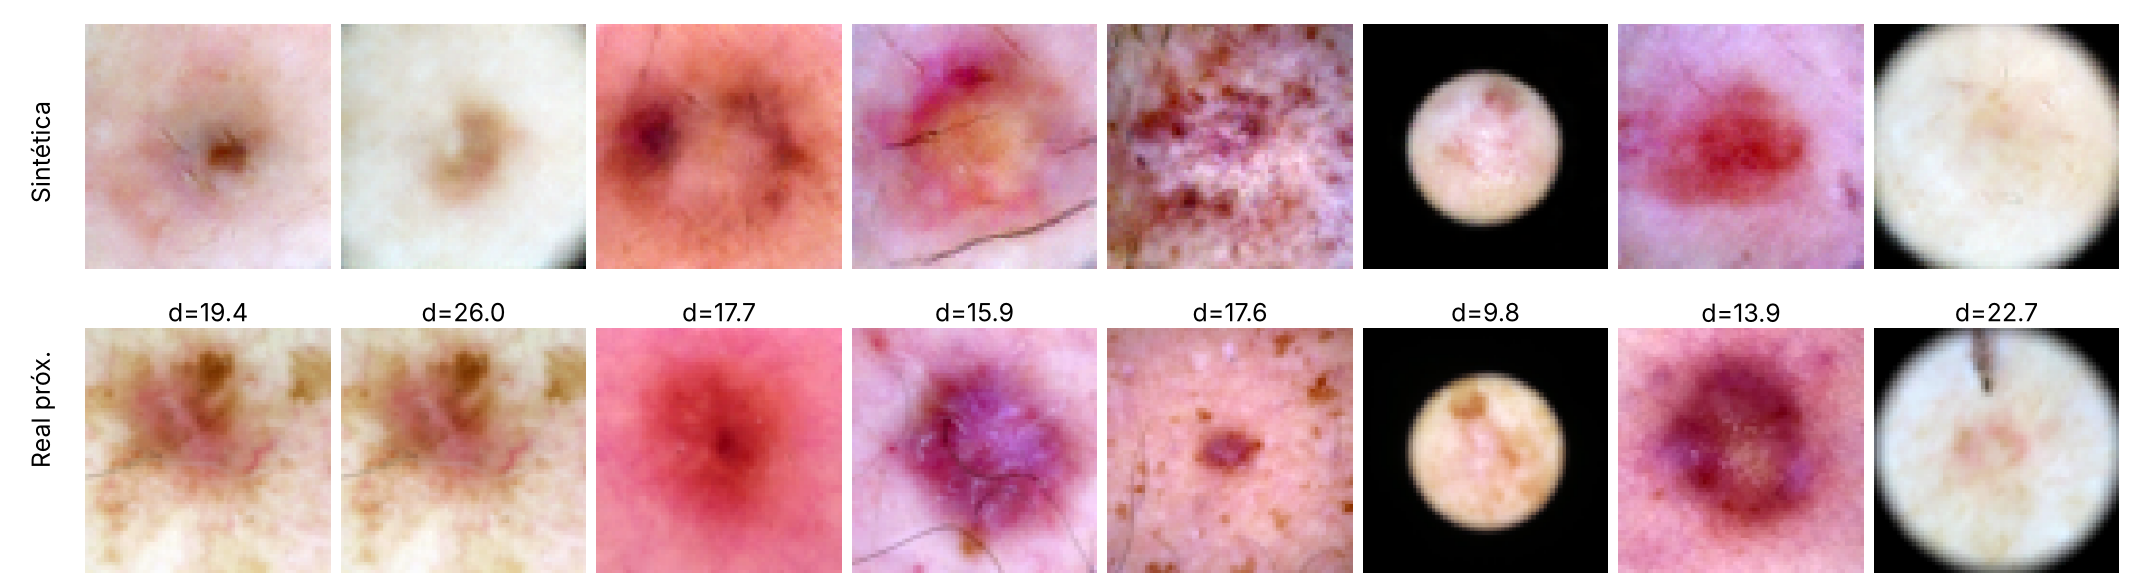
\includegraphics[width=\columnwidth]{fig_nn.png}
\caption{Imagens sintéticas (linha superior) e a respectiva DF de treino mais próxima nas \textit{features} da ResNet18 (inferior), com a distância euclidiana $d$ (\textit{fold}~0).}
\label{fig:nn}
\end{figure}

\section{Conclusão}
Com partições sem vazamento, validação cruzada e controles de rebalanceamento, uma DCGAN treinada com cerca de 155 imagens de dermatofibroma por \textit{fold} gerou imagens de cor e forma plausíveis, porém borradas e pouco diversas (FID de 191 a 225), sem indício consistente de memorização. Essas imagens não melhoraram a detecção do DF, com variação de recall de \pl0,008 (intervalo de \mn0,026 a \pl0,040) sobre o \textit{baseline} e nenhum ganho mensurável sobre os controles. Repetir imagens reais e ponderar a perda, por outro lado, elevaram o recall em 0,071 e 0,061, o que mostra que parte do benefício atribuído ao aumento de dados vem do simples rebalanceamento.

Para o objetivo de equidade, o resultado sustenta duas recomendações. Dados sintéticos devem ser avaliados contra controles de rebalanceamento, e sua qualidade e diversidade devem ser medidas antes do uso. Como próximos passos, sugerem-se treinos mais longos e em maior resolução, filtragem das imagens sintéticas, mais classes raras e análise por subgrupo demográfico. Por fim, imagens sintéticas devem passar por validação clínica humana antes de qualquer uso em sistemas médicos em produção.

\begin{thebibliography}{00}
\bibitem{tschandl2018ham10000}
P.~Tschandl, C.~Rosendahl, and H.~Kittler, ``The HAM10000 dataset, a large collection of multi-source dermatoscopic images of common pigmented skin lesions,'' \emph{Scientific Data}, vol.~5, art.~180161, 2018.

\bibitem{codella2018skin}
N.~C.~F. Codella \emph{et al.}, ``Skin lesion analysis toward melanoma detection: A challenge at the 2017 International Symposium on Biomedical Imaging (ISBI), hosted by the International Skin Imaging Collaboration (ISIC),'' in \emph{Proc. IEEE ISBI}, 2018, pp. 168--172.

\bibitem{combalia2019bcn20000}
M.~Combalia \emph{et al.}, ``BCN20000: Dermoscopic lesions in the wild,'' arXiv:1908.02288, 2019.

\bibitem{daneshjou2022disparities}
R.~Daneshjou \emph{et al.}, ``Disparities in dermatology AI performance on a diverse, curated clinical image set,'' \emph{Science Advances}, vol.~8, no.~32, art.~eabq6147, 2022.

\bibitem{goodfellow2014generative}
I.~Goodfellow \emph{et al.}, ``Generative adversarial nets,'' in \emph{Advances in Neural Information Processing Systems (NIPS)}, 2014, pp. 2672--2680.

\bibitem{frid2018gan}
M.~Frid-Adar, I.~Diamant, E.~Klang, M.~Amitai, J.~Goldberger, and H.~Greenspan, ``GAN-based synthetic medical image augmentation for increased CNN performance in liver lesion classification,'' \emph{Neurocomputing}, vol.~321, pp. 321--331, 2018.

\bibitem{buda2018systematic}
M.~Buda, A.~Maki, and M.~A. Mazurowski, ``A systematic study of the class imbalance problem in convolutional neural networks,'' \emph{Neural Networks}, vol.~106, pp. 249--259, 2018.

\bibitem{radford2016unsupervised}
A.~Radford, L.~Metz, and S.~Chintala, ``Unsupervised representation learning with deep convolutional generative adversarial networks,'' in \emph{Proc. ICLR}, 2016.

\bibitem{kingma2015adam}
D.~P. Kingma and J.~Ba, ``Adam: A method for stochastic optimization,'' in \emph{Proc. ICLR}, 2015.

\bibitem{salimans2016improved}
T.~Salimans \emph{et al.}, ``Improved techniques for training GANs,'' in \emph{Advances in Neural Information Processing Systems (NIPS)}, 2016, pp. 2234--2242.

\bibitem{zhao2020differentiable}
S.~Zhao, Z.~Liu, J.~Lin, J.-Y. Zhu, and S.~Han, ``Differentiable augmentation for data-efficient GAN training,'' in \emph{Advances in Neural Information Processing Systems (NeurIPS)}, vol.~33, 2020, pp. 7559--7570.

\bibitem{yazici2019unusual}
Y.~Yaz{\i}c{\i}, C.-S. Foo, S.~Winkler, K.-H. Yap, G.~Piliouras, and V.~Chandrasekhar, ``The unusual effectiveness of averaging in GAN training,'' in \emph{Proc. ICLR}, 2019.

\bibitem{heusel2017gans}
M.~Heusel, H.~Ramsauer, T.~Unterthiner, B.~Nessler, and S.~Hochreiter, ``GANs trained by a two time-scale update rule converge to a local Nash equilibrium,'' in \emph{Advances in Neural Information Processing Systems (NIPS)}, 2017, pp. 6626--6637.

\bibitem{seitzer2020pytorchfid}
M.~Seitzer, ``pytorch-fid: FID score for PyTorch,'' version 0.3.0, 2020. [Online]. Available: https://github.com/mseitzer/pytorch-fid

\bibitem{he2016deep}
K.~He, X.~Zhang, S.~Ren, and J.~Sun, ``Deep residual learning for image recognition,'' in \emph{Proc. IEEE CVPR}, 2016, pp. 770--778.
\end{thebibliography}
\end{document}